\documentclass[a4paper]{article} 
\addtolength{\hoffset}{-2.25cm}
\addtolength{\textwidth}{4.5cm}
\addtolength{\voffset}{-3.25cm}
\addtolength{\textheight}{5cm}
\setlength{\parskip}{0pt}
\setlength{\parindent}{0in}

\usepackage[square,sort,comma,numbers]{natbib}
\usepackage{blindtext} % Package to generate dummy text
\usepackage{charter} % Use the Charter font
\usepackage[utf8]{inputenc} % Use UTF-8 encoding
\usepackage{microtype} % Slightly tweak font spacing for aesthetics
\usepackage{amsthm, amsmath, amssymb} % Mathematical typesetting
\usepackage{float} % Improved interface for floating objects
\usepackage{hyperref} % For hyperlinks in the PDF
\usepackage{graphicx, multicol} % Enhanced support for graphics
\usepackage{xcolor} % Driver-independent color extensions
\usepackage{pseudocode} % Environment for specifying algorithms in a natural way
\usepackage[yyyymmdd]{datetime} % Uses YEAR-MONTH-DAY format for dates

\usepackage{fancyhdr} % Headers and footers
\pagestyle{fancy} % All pages have headers and footers
\fancyhead{}\renewcommand{\headrulewidth}{0pt} % Blank out the default header
\fancyfoot[L]{} % Custom footer text
\fancyfoot[C]{} % Custom footer text
\fancyfoot[R]{\thepage} % Custom footer text
\newcommand{\note}[1]{\marginpar{\scriptsize \textcolor{red}{#1}}} % Enables comments in red on margin

%----------------------------------------------------------------------------------------

\usepackage{amsmath}
\usepackage{bbm}
\usepackage{dsfont}

\newcommand\independent{\protect\mathpalette{\protect\independenT}{\perp}}
\def\independenT#1#2{\mathrel{\rlap{$#1#2$}\mkern2mu{#1#2}}}


%-------------------------------
%	TITLE VARIABLES (identify your work!)
%-------------------------------

\newcommand{\yourname}{Javier Martinez Hernandez} % replace YOURNAME with your name
%\newcommand{\yournetid}{Student ID: 251054234} % replace YOURNETID with your NetID
\newcommand{\youremail}{fmarti23@uwo.ca} % replace YOUREMAIL with your email
%\newcommand{\assignmentnumber}{1} % replace X with assignment number
\newcommand{\deliverynumber}{1} % replace X with assignment number

\begin{document}

%-------------------------------
%	TITLE SECTION (do not modify unless you really need to)
%-------------------------------
\fancyhead[C]{}
\hrule \medskip
\begin{minipage}{0.295\textwidth} 
\raggedright
\footnotesize
\yourname \hfill\\ 
%\yournetid \hfill\\ 
\youremail
\end{minipage}
\begin{minipage}{0.4\textwidth} 
\centering 
\large 
ADV. MACRO II % \assignmentnumber\\ 
\normalsize 
Problem Set \deliverynumber\\ 
\end{minipage}
\begin{minipage}{0.295\textwidth} 
\raggedleft
\today\hfill\\
\end{minipage}
\medskip\hrule 
\bigskip


%-------------------------------
%	ASSIGNMENT CONTENT (add your responses)
%-------------------------------

\section{PART I}

Consider the Neo-Classical growth model. Time is discrete and goes on forever. There is a representative agent that derives utility only from consumption and discounts future utility at a rate $\beta$. The agent owns $k_0$ units of capital and has an endowment of time that can be used for labor or leisure every period. The time endowment is normalized to 1. There is a representative firm that hires labor and rents capital to produce using a constant returns to scale technology. Capital rental rate is $r$ and the wage is $w$. Capital depreciates fully after use (i.e. $\rho = 1$).


\begin{enumerate}
\item[1.] Define a competitive equilibrium for this economy.\\~\

A competitive equilibrium is a sequence of prices $\{p_{t},w_{t}, r_{t}\}^{\infty}_{t=0}$, allocations for the firm $\{ k^{d}_{t}, n^{d}_{t}, y_{t} \}^{\infty}_{t=0}$ and allocations for the household $ \{ c_{t}, i_{t}, x_{t+1}, k^{s}_{t}, n^{s}_{t} \}^{\infty}_{t=0}$ such that
\begin{itemize}
\item Given prices $\{p_{t},w_{t}, r_{t}\}^{\infty}_{t=0}$, the allocation of the representative firm solves: 
\begin{align*}
\max_{ \{ y_{t}, k_{t}, n_{t} \}^{\infty}_{t=0} } \sum^{\infty}_{t=0} p_{t}(y_{t}- r_{t}k_{t} - w_{t}n_{t})
\end{align*}
subject to:
\begin{align*}
y_{t} = F(k_{t}, n_{t}) \forall t\geq 0 \\
y_{t},k_{t},n_{t} \geq 0
\end{align*}


\item Given prices $\{p_{t},w_{t}, r_{t}\}^{\infty}_{t=0}$, the allocation of the representative household solves: 
\begin{align*}
\max_{ \{ c_{t}, i_{t}, x_{t+1}, k^{s}_{t}, n^{s}_{t} \}^{\infty}_{t=0}} \sum^{\infty}_{t=0} \beta^{t} U(c_{t}) \\
subject \: \: to \\
\sum^{\infty}_{t=0} p_{t}(c_{t} + i_{t}) \leq \sum^{\infty}_{t=0} p_{t}(r_{t}k_{t} + w_{t}n_{t}) + \pi \\
x_{t+1} = (1-\delta)x_{t} + i_{t}, \: \: \: \forall t \geq 0 \\
0 \leq n_{t} \leq 1, \: 0 \leq k_{t} \leq x_{t}, \: \forall	t \geq 0\\
c_{t}, x_{t+1} \geq 0, \: \forall t \geq 0 \\
x_{0} \: \: given
\end{align*}

\item Markets clear
\begin{align*}
y_{t} = c_{t} + i_{t} \: \: \: Goods \: \: market \\
k^{d}_{t} = k^{s}_{t} \: \: \: Capital \: \: market \\
n^{d}_{t} = n^{s}_{t} \: \: \: Labor \: \: market
\end{align*}
\end{itemize}


\item[2.] Define the social planner's problem for this economy\\~\

The social planner problem is to maximize the utility for the representative consumer subject to the feasibility constraint. By substituting out first the feasibility constraint into the utility function, we can pose the following problem for the social planner:\\~\
\begin{align*}
\max_{ \{ k_{t+1} \}^{\infty}_{t=0} } \sum^{\infty}_{t=0} \beta^{t} U(f(k_{t} - k_{t+1}) \\
0 \leq k_{t+1} \leq f(k_{t}) \\
k_{0} = \bar{k}_{0} >0 \: \: given
\end{align*}


\item[3.] Show that the equilibrium allocation of consumption, capital, and labor coincides with those of the planner’s.\\~\
We can start from the first order condition of the competitive equilibrium:
\begin{align*}
-u'(c_t) + \beta u'(c_{t+1})r_t = 0
\end{align*}
And in this economy we know that $F(k_t, l_t) = zk_t^{\alpha}l_t^{1-\alpha}$, with depreciation rate $\delta = 1$. If we do $f(k_t, l_t) = F(k_t, l_t) + (1-\delta)k_t$ with $l_t = 1$ due to inelastic labor supply, we can rewrite the f.o.c. from the utility maximization problem as:
\begin{align*}
-u'(c_t) + \beta u'(c_{t+1})f'(k_t) = 0
\end{align*}
Furthermore with the goods market clearing condition $c_t = f(k_t) - k_{t+1}$, we can substitute out into the f.o.c of the competitive equilibrium:
\begin{align*}
-u'(f(k_t) - k_{t+1}) + \beta u'(f(k_{t+1}) - k_{t+2})f'(k_{t+1}) = 0
\end{align*}
which is the first order condition of Social Planners' sequential formulation. Furthermore,  the TVC of the social planner problem is $\lim_{t \rightarrow \infty} \lambda_t k_{t+1} = 0$, where $\lambda_t$ is the Lagrange multiplier of the resource constraint. In the competitive equilibrium formulation the TVC is  $\lim_{t \rightarrow \infty} p_t k_{t+1} = 0$. Let $\mu$ be the associated Lagrange multiplier on the budget constraint of the household in the CE formulation and it is always positive due to local non-satiation (i.e. budget constraint is binding). Then:
\begin{align*}
\lim_{t \rightarrow \infty} p_t k_{t+1} = 0\\
& = \frac{1}{\mu} \lim_{t \rightarrow \infty} \beta^{t} u'(f(k_t)-k_{t+1})f'(k_t)k_t = 0
\end{align*}
Which is the same TVC as for the social planners problem. \\~\

Hence we can state that an allocation of capital (or a sequence of capital) $k_{t+1}$ satisfies the necessary and sufficient conditions for being a Pareto optimal allocation, if and only if it satisfies the necessary and sufficient conditions for being part of a CE, subject to the TVC being satisfied in both problems.
\item[4.] Pose the planner’s dynamic programming problem. Write down the appropriate Bellman equation.\\~\
\begin{align*}
V(k) = \max_{0\leq k' \leq f(k)} \left\lbrace U(f(k) - k') + \beta V(k') \right\rbrace
\end{align*}
\item[5.].Assume that the utility of the consumer is $u(c) = log(c)$ and that the production function is $f(k,l) = zk^\alpha l^{1-\alpha}$. Solve the planner's dynamic programming problem.\\~\ 
First note that labor is supplied inelastically. This reduces our production function to $f(k,1) = zk^\alpha $. \\~\
To solve by hand I use the method of undertermined coefficients, and I propose the following guess:
\begin{equation}
V(k) = \Theta+ \Omega ln(k)
\end{equation}
where $\Theta$, $\Omega$ are undetermined coefficients that we will solve for. Given that the constraints on $k'$ do not bind, the objective funciton is strictly concave and the constraint set is compact for $k'$, for any given $k$, By the Weierstrass theorem, the FOC for $k'$ is sufficient for the unique solution.\\~\
\begin{align*}
V(k) = \max_{0\leq k' \leq f(k)} \left\lbrace log(zk^\alpha - k') + \beta(\Theta+ \Omega log(k')) \right\rbrace
\end{align*}

The first order condition is:
\begin{align*}
-\frac{1}{zk^\alpha - k'} = \frac{\beta \Omega}{k'}
\end{align*}
Which implies 
\begin{equation*}
k' = \frac{\beta \Omega z k^\alpha}{1+\beta \Omega}
\end{equation*}

After evaluating the optimal solution in the RHS, we obtain that 
\begin{align*}
\Omega = \frac{\alpha}{1-\alpha \beta}
\end{align*}
and
\begin{align*}
\Theta=\frac{1}{1-\beta} \left[ \frac{\alpha \beta}{1-\alpha \beta} log(\alpha \beta) + log(1-\alpha \beta) \right]
\end{align*}


This implies that after substituting B into our first order condition for optimality ($k' = \phi(k)$): 
\begin{align*}
\phi(k) = \frac{\beta \Omega k^\alpha}{1+\beta \Omega} \\
\end{align*}

\begin{align}
\phi(k) = \alpha \beta z k^\alpha
\end{align}


\item[6.]Use the solution to the planner’s problem to obtain the steady state value of $\left[c,k,r,w,y\right]$ \\~\

Employing the principle of optimality, we know that the dynamic programming problem for the Social Planner can be used as a solution for the sequential formulation. With that, once we know the equilibrium sequence of capital stocks $\left[ k_{t+1} \right]^{\infty}_{t=0} $, we can back out the equilibrium allocations.

From our recursive solution we know that $k'=\alpha \beta z k^{\alpha}$, which implies that in the steady state $k* = (\alpha \beta z)^{\frac{1}{1-\alpha}}$.



Then, 
\begin{itemize}
\item $c* = f(k*, 1) - k_{*} = z(k*)^{\alpha} - k* = z (\alpha \beta z)^{\frac{\alpha}{1-\alpha}} - (\alpha \beta)^{\frac{1}{1-\alpha}}$
\item $y* = f(k*, 1) = z(k*)^{\alpha} = z(\alpha \beta z)^{\frac{\alpha}{1-\alpha}}$
\item $r* = \frac{1}{\beta}$ 
\item $w* = (1-\alpha)z(\alpha \beta z)^{\frac{\alpha}{1-\alpha}}$
\end{itemize}


\item[7.] For this exercise assume that $\alpha = 1/3$, z = 1. Use the solution to the planner’s problem to obtain the path of $\left\lbrace c, k, r, w, y \right\rbrace$ starting from the steady state after the following changes: \\~\

So, if I am understanding correctly the question what we are asked to do here are impulse response functions. Since we know the steady state values of the variables in the model $\left\lbrace c, k, r, w, y \right\rbrace$, we need to calculate the steady state values with the information given, and then graph the response.  

\begin{enumerate}
\item[I.] Capital decreases to 80\%
\begin{itemize}
\item Consumption
\begin{center}
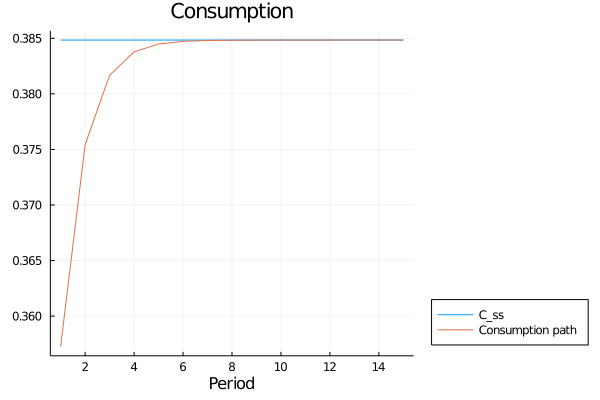
\includegraphics[scale=0.5]{../../../../../github/advmacro_ps/ps1/Figures/consumption.png} 
\end{center}
\clearpage
\item Capital
\begin{center}
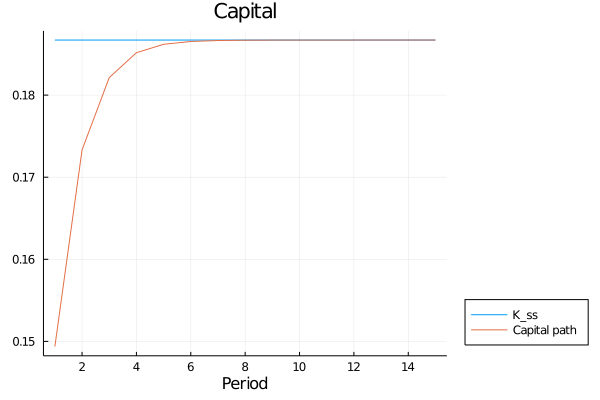
\includegraphics[scale=0.5]{../../../../../github/advmacro_ps/ps1/Figures/capital.png} 
\end{center}
\item Interest Rate
\begin{center}
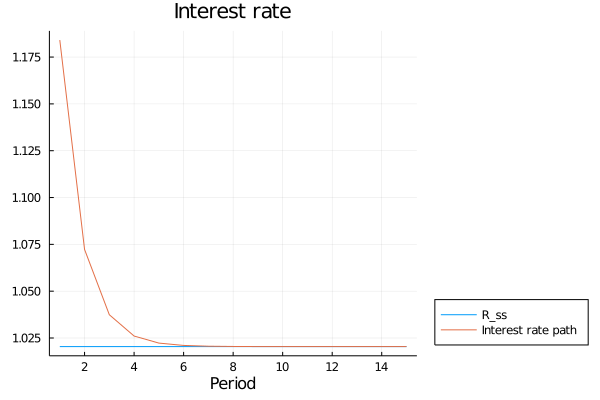
\includegraphics[scale=0.5]{../../../../../github/advmacro_ps/ps1/Figures/interest_rate.png} 
\end{center}
\item Wage
\begin{center}
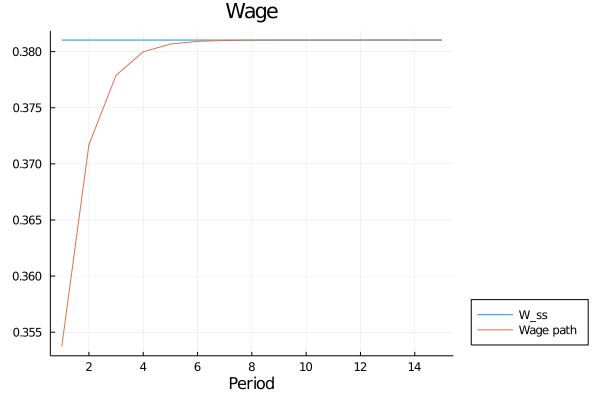
\includegraphics[scale=0.5]{../../../../../github/advmacro_ps/ps1/Figures/wage.png} 
\end{center}
\clearpage
\item Production
\begin{center}
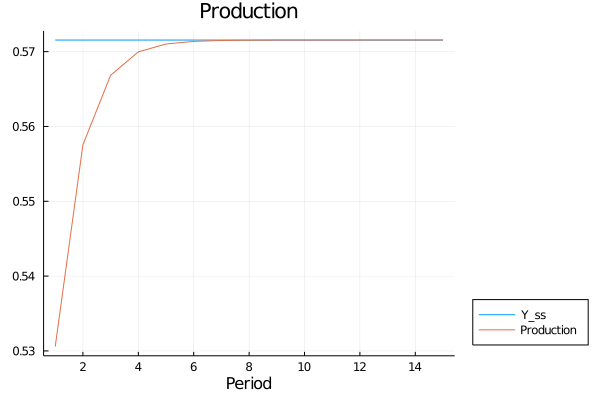
\includegraphics[scale=0.5]{../../../../../github/advmacro_ps/ps1/Figures/production.png} 
\end{center}

\end{itemize}

\item[II.] Productivity increases permanently by 5\%
\begin{itemize}
\item Consumption
\begin{center}
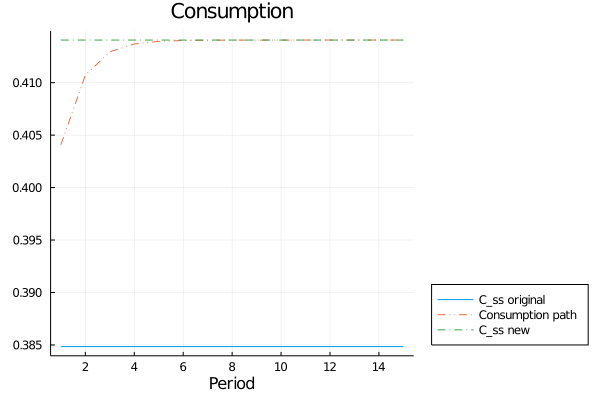
\includegraphics[scale=0.5]{../../../../../github/advmacro_ps/ps1/Figures/consumption_b.png} 
\end{center}
\item Capital
\begin{center}
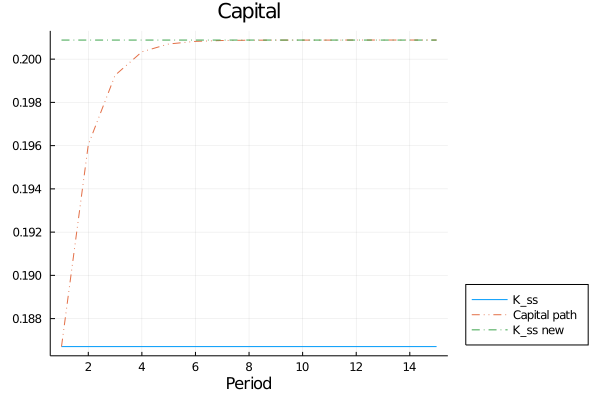
\includegraphics[scale=0.5]{../../../../../github/advmacro_ps/ps1/Figures/capital_b.png} 
\end{center}
\clearpage
\item Interest Rate
\begin{center}
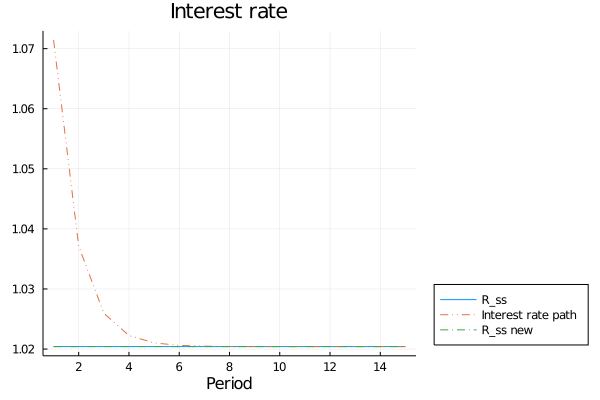
\includegraphics[scale=0.5]{../../../../../github/advmacro_ps/ps1/Figures/interest_rate_b.png} 
\end{center}
\item Wage
\begin{center}
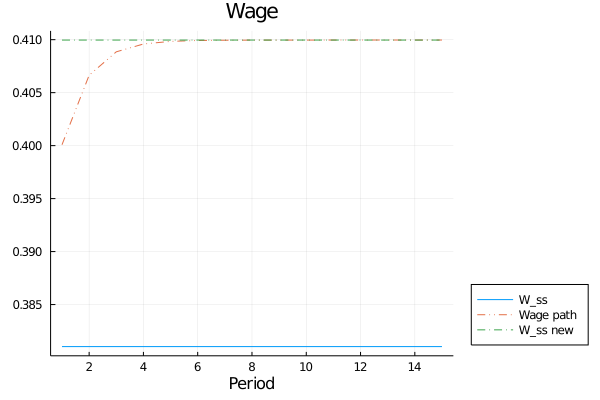
\includegraphics[scale=0.5]{../../../../../github/advmacro_ps/ps1/Figures/wage_b.png} 
\end{center}
\item Production
\begin{center}
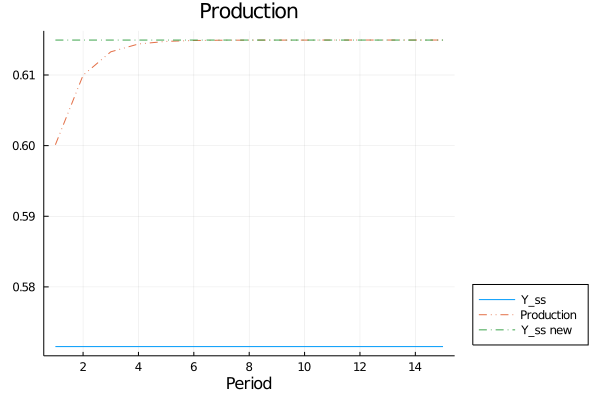
\includegraphics[scale=0.5]{../../../../../github/advmacro_ps/ps1/Figures/production_b.png} 
\end{center}

\end{itemize}
\end{enumerate}





\end{enumerate}







%------------------------------------------------
%
%\bibliographystyle{acm}
%\bibliography{references} % citation records are in the references.bib document

\end{document}
